% IN THE NAME OF GOD
% LaTeX Problem Set Template by Sachin Padmanabhan edited by Ali Heydari
% I created this when I was a freshman in CS 103,
% and I continue to use it to this day.
%
% Hope you enjoy!
%
% There may be problems with this template.
% If so, feel free to contact me.
%

\documentclass[a4paper]{article}
\usepackage{amsmath}
\usepackage{amssymb}
\usepackage{amsthm}
\usepackage{amssymb}
\usepackage{mathdots}
\usepackage[pdftex]{graphicx}
\usepackage{fancyhdr}
\usepackage[margin=1in]{geometry}
\usepackage{multicol}
\usepackage{bm}
\usepackage{listings}
\PassOptionsToPackage{usenames,dvipsnames}{color}  %% Allow color names
\usepackage{pdfpages}
\usepackage{algpseudocode}
\usepackage{tikz}
\usepackage{enumitem}
\usepackage[T1]{fontenc}
\usepackage{inconsolata}
\usepackage{framed}
\usepackage{wasysym}
\usepackage[thinlines]{easytable}
\usepackage{hyperref}
\usepackage{dsfont}


\usepackage{wrapfig}
\setlength{\intextsep}{0pt}
\setlength{\columnsep}{0pt}
\usepackage{subcaption}
\usepackage{graphicx}
\graphicspath{ {images/} }

\hypersetup{
    colorlinks=true,
    linkcolor=blue,
    filecolor=magenta,
    urlcolor=blue,
}

\title{
\textsc{Iran university of science and technology} \\ [25pt] % Your university, school and/or department name(s)
Discrete mathematics\\Problem Set \#4 \\
}
\author{Ali Heydari}
\date{\today}

\lhead{Ali Heydari}
\chead{Problem Set \#4}
\rhead{\today}
\lfoot{}
\cfoot{Discrete mathematics --- Spring 2018}
\rfoot{\thepage}

\newcommand{\abs}[1]{\lvert #1 \rvert}
\newcommand{\absfit}[1]{\left\lvert #1 \right\rvert}
\newcommand{\norm}[1]{\left\lVert #1 \right\rVert}
\newcommand{\eval}[3]{\left[#1\right]_{#2}^{#3}}
\renewcommand{\(}{\left(}
\renewcommand{\)}{\right)}
\newcommand{\floor}[1]{\left\lfloor#1\right\rfloor}
\newcommand{\ceil}[1]{\left\lceil#1\right\rceil}
\newcommand{\pd}[1]{\frac{\partial}{\partial #1}}
\newcommand{\inner}[1]{\langle#1\rangle}
\newcommand{\cond}{\bigg|}
\newcommand{\rank}[1]{\mathbf{rank}(#1)}
\newcommand{\range}[1]{\mathbf{range}(#1)}
\newcommand{\nullsp}[1]{\mathbf{null}(#1)}
\newcommand{\repr}[1]{\left\langle#1\right\rangle}

\DeclareMathOperator{\Var}{Var}
\DeclareMathOperator{\tr}{tr}
\DeclareMathOperator{\Tr}{\mathbf{Tr}}
\DeclareMathOperator{\diag}{\mathbf{diag}}
\DeclareMathOperator{\dist}{\mathbf{dist}}
\DeclareMathOperator{\prob}{\mathbf{prob}}
\DeclareMathOperator{\dom}{\mathbf{dom}}
\DeclareMathOperator{\E}{\mathbf{E}}
\DeclareMathOperator{\R}{\mathbb{R}}
\DeclareMathOperator{\var}{\mathbf{var}}
\DeclareMathOperator{\quartile}{\mathbf{quartile}}
\DeclareMathOperator{\conv}{\mathbf{conv}}
\DeclareMathOperator{\VC}{VC}
\DeclareMathOperator*{\argmax}{arg\,max}
\DeclareMathOperator*{\argmin}{arg\,min}
\DeclareMathOperator{\Ber}{Bernoulli}
\DeclareMathOperator{\NP}{\mathbf{NP}}
\DeclareMathOperator{\coNP}{\mathbf{coNP}}
\DeclareMathOperator{\TIME}{\mathsf{TIME}}
\DeclareMathOperator{\polytime}{\mathbf{P}}
\DeclareMathOperator{\PH}{\mathbf{PH}}
\DeclareMathOperator{\SIZE}{\mathbf{SIZE}}
\DeclareMathOperator{\ATIME}{\mathbf{ATIME}}
\DeclareMathOperator{\SPACE}{\mathbf{SPACE}}
\DeclareMathOperator{\ASPACE}{\mathbf{ASPACE}}
\DeclareMathOperator{\NSPACE}{\mathbf{NSPACE}}
\DeclareMathOperator{\Z}{\mathbb{Z}}
\DeclareMathOperator{\N}{\mathbb{N}}
\DeclareMathOperator{\EXP}{\mathbf{EXP}}
\DeclareMathOperator{\NEXP}{\mathbf{NEXP}}
\DeclareMathOperator{\NTIME}{\mathbf{NTIME}}
\DeclareMathOperator{\DTIME}{\mathbf{DTIME}}
\DeclareMathOperator{\poly}{poly}
\DeclareMathOperator{\BPP}{\mathbf{BPP}}
\DeclareMathOperator{\ZPP}{\mathbf{ZPP}}
\DeclareMathOperator{\RP}{\mathbf{RP}}
\DeclareMathOperator{\coRP}{\mathbf{coRP}}
\DeclareMathOperator{\BPL}{\mathbf{BPL}}
\DeclareMathOperator{\IP}{\mathbf{IP}}
\DeclareMathOperator{\PSPACE}{\mathbf{PSPACE}}
\DeclareMathOperator{\NPSPACE}{\mathbf{NPSPACE}}
\DeclareMathOperator{\SAT}{\mathsf{SAT}}
\DeclareMathOperator{\NL}{\mathbf{NL}}
\DeclareMathOperator{\PCP}{\mathbf{PCP}}
\DeclareMathOperator{\PP}{\mathbf{PP}}
\DeclareMathOperator{\cost}{cost}
\let\Pr\relax
\DeclareMathOperator*{\Pr}{\mathbf{Pr}}

\definecolor{shadecolor}{gray}{0.95}

\theoremstyle{plain}
\newtheorem*{lem}{Lemma}

\theoremstyle{plain}
\newtheorem*{claim}{Claim}

\theoremstyle{definition}
\newtheorem*{answer}{Answer}

\newtheorem{theorem}{Theorem}[section]
\newtheorem*{thm}{Theorem}
\newtheorem{corollary}{Corollary}[theorem]
\newtheorem{lemma}[theorem]{Lemma}

\renewcommand{\headrulewidth}{0.4pt}
\renewcommand{\footrulewidth}{0.4pt}

\setlength{\parindent}{0pt}

\pagestyle{fancy}

\renewcommand{\thefootnote}{\fnsymbol{footnote}}

\begin{document}

\maketitle

\section{Prove the sequence}
Consider the sequence defined recursively by:
\begin{align*}
   & a_0 = 1 \\
   & a_n = a_{n-1} + a_{n-2} + \dots + a_0 +1
\end{align*}
Prove that $a_n=2^n$ by strong induction.

\begin{shaded}
\begin{answer}
\begin{proof}
PROOF HERE.
\end{proof}
\end{answer}
\end{shaded}

\section{Fill the board using  L shaped tiles}
Given a $n$ by $n$ board where $n$ is of form $2k$ where $k \geq 1$ (Basically n is a power of 2 with minimum value as 2). The board has one missing cell (of size $1 \times 1$). Prove that the board can be filled using $L$ shaped tiles.

 A $L$ shaped tile is $2 \times 2$ square with one cell of size $1\times 1$ missing.

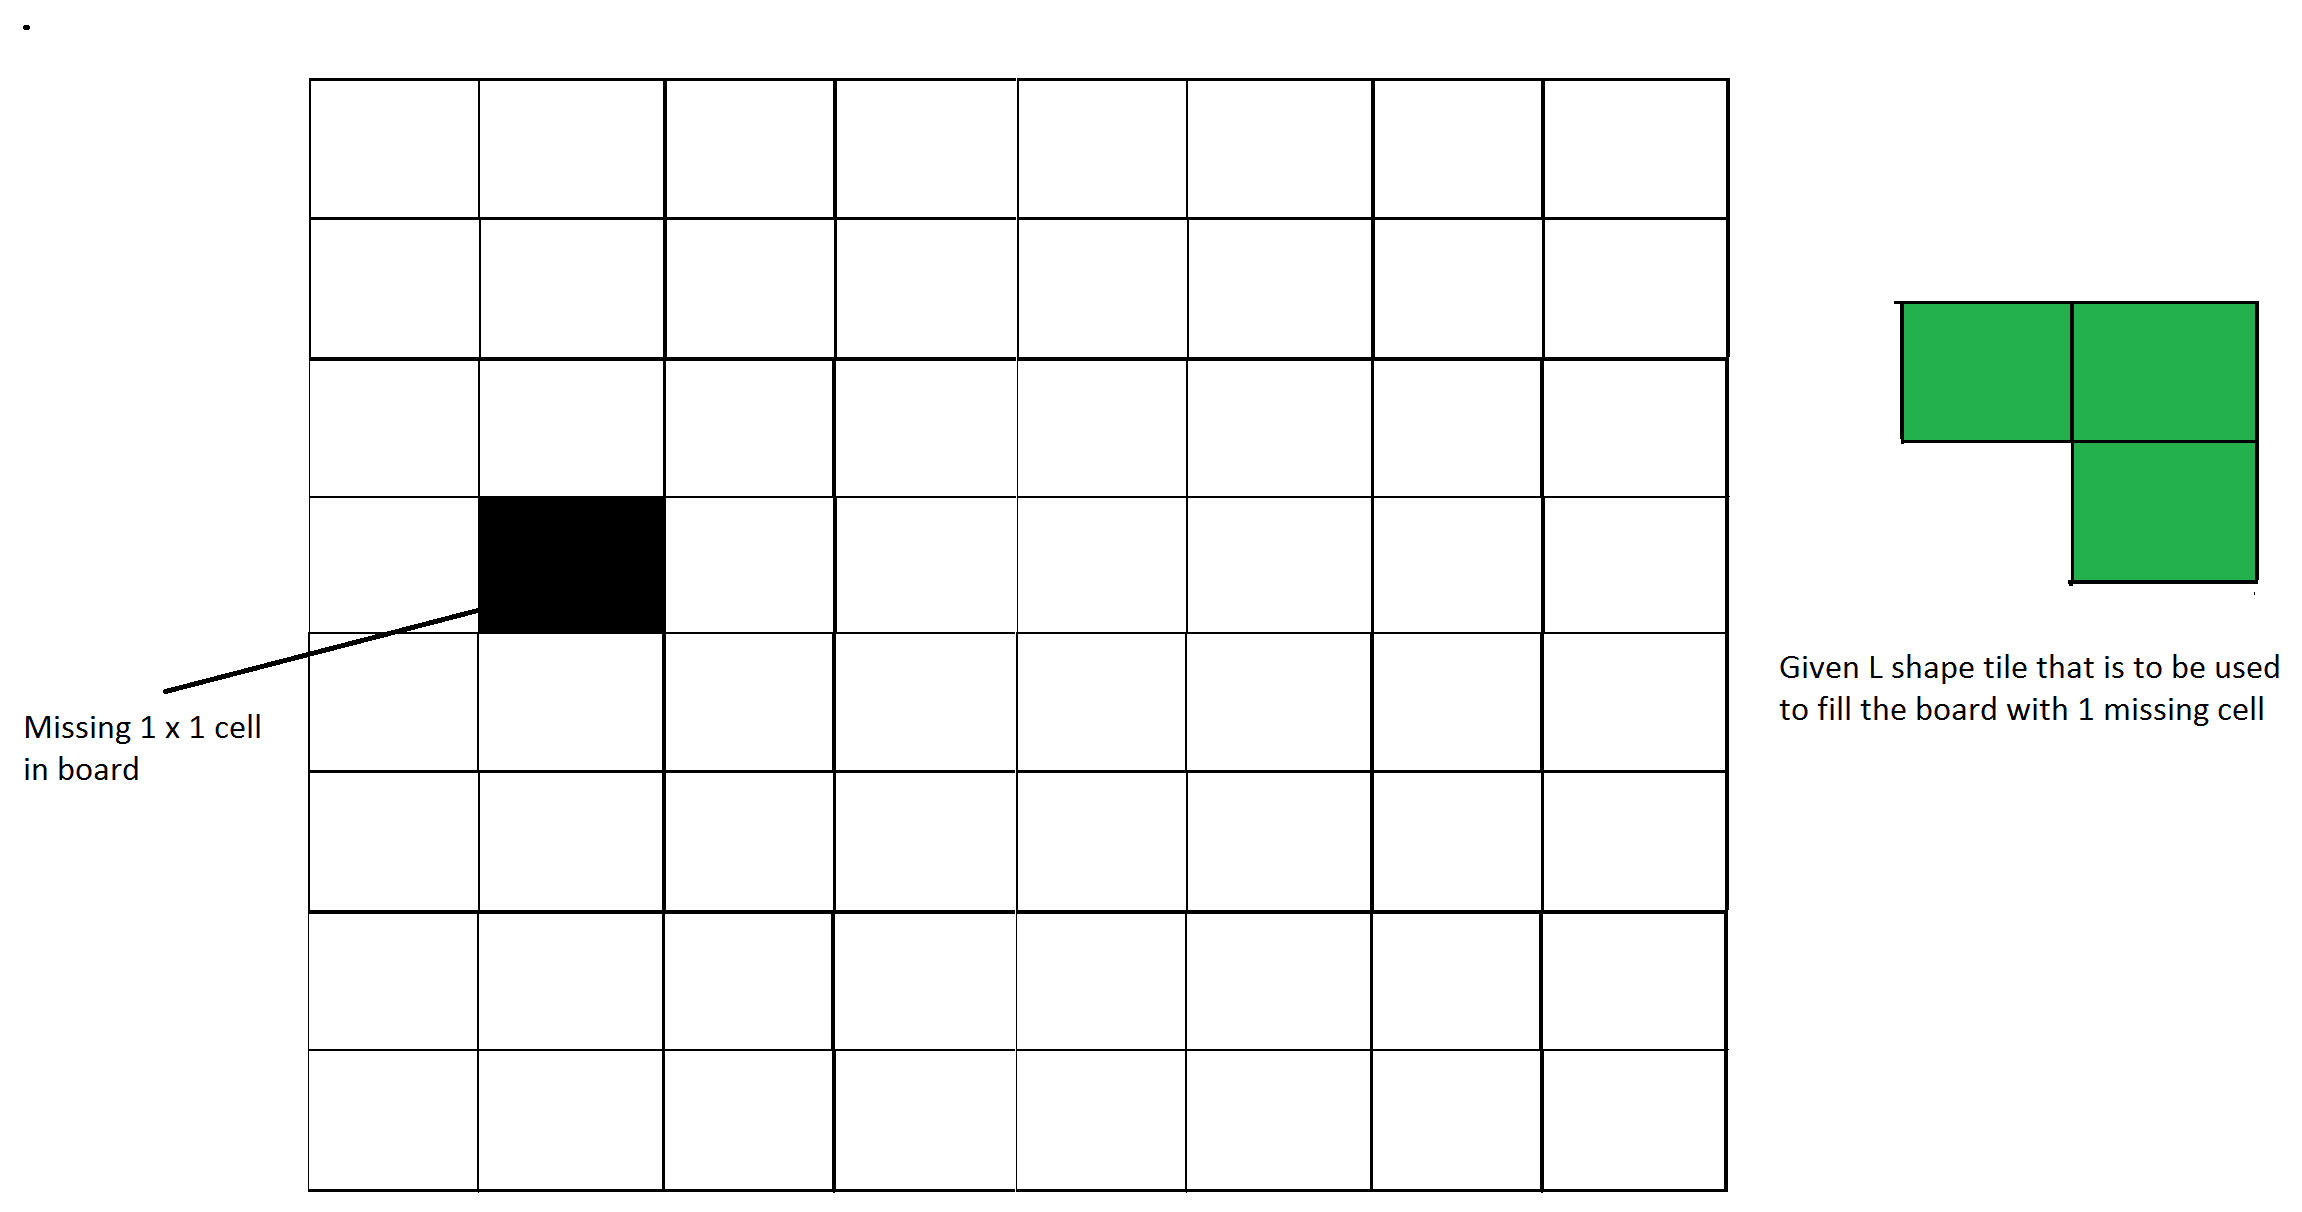
\includegraphics[scale = 0.2]{LShapes}

\begin{shaded}
\begin{answer}
\begin{proof}
PROOF HERE.
\end{proof}
\end{answer}
\end{shaded}

\section{Prime number and positive number}
prove that every positive integer $n$, $n \geq 2$, can be expressed as the product of one or more prime numbers.
\begin{shaded}
\begin{answer}
\begin{proof}
PROOF HERE.
\end{proof}
\end{answer}
\end{shaded}

\section{The game}
In a game , there are two players and two piles of matches. At each turn, a player removes some (non-zero) number of matches from one of the piles. The player who removes the last match wins.

Prove that if the two piles contain the same number of matches at the start of the game, then the second player can always win.

\begin{shaded}
\begin{answer}
\begin{proof}
$$$$

\begin{itemize}
 \item[] {Here's a winning strategy for the second player. Suppose your opponent removes $m$ matches from one pile. You remove $m$ matches from the other pile. Let's prove that this strategy works.
\begin{itemize}

\item[] {Proof by induction on the number of matches $(n)$ in each pile.
\textbf{Base:} If both piles contain 1 match, the first player has only one possible move: remove the last match from one pile. The second player can then remove the last match from the other pile and thereby win.

\textbf{Induction:} Suppose that the second player can win any game that starts with two piles of $n$ matches, where $n$ is any value from 1 through $k$. We need to show that this is true if $n = k + 1$. So, suppose that both piles contain $k + 1$ matches. A legal move by the first player involves removing $j$ matches from one pile, 1Or, in some variations, loses. There seem to be several variations of this game.

where $0 \leq j \leq k + 1$. The piles then contain $k + 1$ matches and $k + 1 − j$ matches. The second player can now remove $j$ matches from the other pile. This leaves us with two piles of $k+1−j$ matches. If $j = k+1$, then the second player wins. If $j < k + 1$, then we're now effectively at the start of a game with $k + 1 − j$ matches in each pile. Since $1 \leq k +1−j \leq k$, we know by the induction hypothesis that the second player can win the game.}
\end{itemize}

The induction step in this proof uses the fact that our claim $P(n)$ is true for a smaller value of $n$. But since we can't control how many matches the first player removes, we don't know how far back we have look in the sequence of earlier results $P(1) . . .P(k)$. Our previous proof about postage can be rewritten so as to avoid strong induction. It's less clear how to rewrite proofs like this Nim example.}
\end{itemize}
\end{proof}
\end{answer}
\end{shaded}

\section{ATM Machine}
Suppose an ATM machine has only $\$2$ and $\$5$ bills.
Claim: The ATM can generate any output amount $n \geq 4$.
Prove the claim.
\begin{shaded}
\begin{answer}
\begin{proof}
\textbf{Base case}: $n = 4$. Two \$2 bills.

\textbf{Induction step}: suppose the machine can already handle $n \geq 4$ dollars.
How do we proceed for $n+1$ dollars?

\textbf{Case 1: }  The $n$ dollar output contains a \$5. Then we can replace the \$5 by three \$2's to get $ n+1$ dollars.
 
 \textbf{Case 2: } The $n$ dollar output contains only \$2 bills. Since $n \geq 4$, there must be at least two \$2 bills. Remove two, and replace them by one \$5.

\end{proof}
\end{answer}
\end{shaded}

\section{Colored computers}
We have $n$ computers ($n \geq 4$), each pair of them are connected by a wire, each wire is colored in blue, red, yellow or green. At least there is a wire colored in each color.

Prove that we can choose a number of computers so that the wires connecting computers, include exactly 3 different colors.

\begin{shaded}
\begin{answer}
\begin{proof}
PROOF HERE.
\end{proof}
\end{answer}
\end{shaded}


\end{document} 